% A LaTeX (non-official) template for ISAE projects reports
% Copyright (C) 2014 Damien Roque
% Version: 0.2
% Author: Damien Roque <damien.roque_AT_isae.fr>

% Template adapted for English reports by:
% Johannes Wasmer (JW)

\documentclass[a4paper,12pt, openany]{book} %openany: chapters start on any
                                %page, not just odd pages (which creates blank pages)
\usepackage[utf8]{inputenc}
\usepackage[T1]{fontenc}


%%%%%%%%%%%%%%%%%%%%%%%%%%%%%%%%%%%%% 
%%%%%%%%%% TEMPLATE CONFIG %%%%%%%%%%
%%%%%%%%%%%%%%%%%%%%%%%%%%%%%%%%%%%%% 

\renewcommand{\familydefault}{\sfdefault} % use sans serif font for whole document

% \usepackage[frenchb]{babel} % If you write in French
\usepackage[english]{babel} % If you write in English


\usepackage[                    % adapted template: use biber
backend=biber,                  % instead of biblatex
style=alphabetic,
citestyle=authoryear
]{biblatex}
\addbibresource{references.bib} %Imports bibliography file

\usepackage{a4wide}
\usepackage{graphicx}
\graphicspath{{./fig/}{./img/}}
\usepackage{subfig}
\usepackage{tikz}
\usetikzlibrary{shapes,arrows}
\usepackage{pgfplots}
\pgfplotsset{compat=newest}
\pgfplotsset{plot coordinates/math parser=false}
\newlength\figureheight
\newlength\figurewidth
\pgfkeys{/pgf/number format/.cd,
  set decimal separator={,\!},
  1000 sep={\,},
}
\usepackage{ifthen}
\usepackage{ifpdf}
\ifpdf
\usepackage[pdftex]{hyperref}
\else
\usepackage{hyperref}
\fi
\usepackage{color}
\hypersetup{%
  colorlinks=true,
  linkcolor=black,
  citecolor=black,
  urlcolor=black}

\renewcommand{\baselinestretch}{1.05}
\usepackage{fancyhdr}
\pagestyle{fancy}
\fancyfoot{}
\fancyhead[LE,RO]{\bfseries\thepage}
\fancyhead[RE]{\bfseries\nouppercase{\leftmark}}
\fancyhead[LO]{\bfseries\nouppercase{\rightmark}}
\setlength{\headheight}{15pt}

\let\headruleORIG\headrule
\renewcommand{\headrule}{\color{black} \headruleORIG}
\renewcommand{\headrulewidth}{1.0pt}
\usepackage{colortbl}
\arrayrulecolor{black}

\fancypagestyle{plain}{
  \fancyhead{}
  \fancyfoot[C]{\thepage}
  \renewcommand{\headrulewidth}{0pt}
}

\makeatletter
\def\@textbottom{\vskip \z@ \@plus 1pt}
\let\@texttop\relax
\makeatother

\makeatletter
\def\cleardoublepage{\clearpage\if@twoside \ifodd\c@page\else%
  \hbox{}%
  \thispagestyle{empty}%
  \newpage%
  \if@twocolumn\hbox{}\newpage\fi\fi\fi}
\makeatother

\usepackage{amsthm}
\usepackage{amssymb,amsmath,bbm}
\usepackage{array}
\usepackage{bm}
\usepackage{multirow}
\usepackage[footnote]{acronym}


%%%%%%%%%%%%%%%%%%%%%%%%%%%%%%%%%%%%%
%%%%%%%%%% CONFIG JOHANNES %%%%%%%%%%
%%%%%%%%%%%%%%%%%%%%%%%%%%%%%%%%%%%%%

\usepackage{fontawesome}
\usepackage{dashrule}
\usepackage{hyperref}
\hypersetup{
  colorlinks,
  linkcolor={red!50!black},
  citecolor={blue!50!black},
  urlcolor={blue!80!black}
}



%%% Local Variables:
%%% mode: latex
%%% TeX-master: "../report"
%%% End:



\newcommand*{\SET}[1]  {\ensuremath{\mathbf{#1}}}
\newcommand*{\VEC}[1]  {\ensuremath{\boldsymbol{#1}}}
\newcommand*{\FAM}[1]  {\ensuremath{\boldsymbol{#1}}}
\newcommand*{\MAT}[1]  {\ensuremath{\boldsymbol{#1}}}
\newcommand*{\OP}[1]  {\ensuremath{\mathrm{#1}}}
\newcommand*{\NORM}[1]  {\ensuremath{\left\|#1\right\|}}
\newcommand*{\DPR}[2]  {\ensuremath{\left \langle #1,#2 \right \rangle}}
\newcommand*{\calbf}[1]  {\ensuremath{\boldsymbol{\mathcal{#1}}}}
\newcommand*{\shift}[1]  {\ensuremath{\boldsymbol{#1}}}

\newcommand{\eqdef}{\stackrel{\mathrm{def}}{=}}
\newcommand{\argmax}{\operatornamewithlimits{argmax}}
\newcommand{\argmin}{\operatornamewithlimits{argmin}}
\newcommand{\ud}{\, \mathrm{d}}
\newcommand{\vect}{\text{Vect}}
\newcommand{\sinc}{\ensuremath{\mathrm{sinc}}}
\newcommand{\esp}{\ensuremath{\mathbb{E}}}
\newcommand{\hilbert}{\ensuremath{\mathcal{H}}}
\newcommand{\fourier}{\ensuremath{\mathcal{F}}}
\newcommand{\sgn}{\text{sgn}}
\newcommand{\intTT}{\int_{-T}^{T}}
\newcommand{\intT}{\int_{-\frac{T}{2}}^{\frac{T}{2}}}
\newcommand{\intinf}{\int_{-\infty}^{+\infty}}
\newcommand{\Sh}{\ensuremath{\boldsymbol{S}}}
\newcommand{\C}{\SET{C}}
\newcommand{\R}{\SET{R}}
\newcommand{\Z}{\SET{Z}}
\newcommand{\N}{\SET{N}}
\newcommand{\K}{\SET{K}}
\newcommand{\reel}{\mathcal{R}}
\newcommand{\imag}{\mathcal{I}}
\newcommand{\cmnr}{c_{m,n}^\reel}
\newcommand{\cmni}{c_{m,n}^\imag}
\newcommand{\cnr}{c_{n}^\reel}
\newcommand{\cni}{c_{n}^\imag}
\newcommand{\tproto}{g}
\newcommand{\rproto}{\check{g}}
\newcommand{\LR}{\mathcal{L}_2(\SET{R})}
\newcommand{\LZ}{\ell_2(\SET{Z})}
\newcommand{\LZI}[1]{\ell_2(\SET{#1})}
\newcommand{\LZZ}{\ell_2(\SET{Z}^2)}
\newcommand{\diag}{\operatorname{diag}}
\newcommand{\noise}{z}
\newcommand{\Noise}{Z}
\newcommand{\filtnoise}{\zeta}
\newcommand{\tp}{g}
\newcommand{\rp}{\check{g}}
\newcommand{\TP}{G}
\newcommand{\RP}{\check{G}}
\newcommand{\dmin}{d_{\mathrm{min}}}
\newcommand{\Dmin}{D_{\mathrm{min}}}
\newcommand{\Image}{\ensuremath{\text{Im}}}
\newcommand{\Span}{\ensuremath{\text{Span}}}

\newtheoremstyle{break}
{11pt}{11pt}%
{\itshape}{}%
{\bfseries}{}%
{\newline}{}%
\theoremstyle{break}

% \theoremstyle{definition}
\newtheorem{definition}{Definition}[chapter]

% \theoremstyle{definition}
\newtheorem{theorem}{Theorem}[chapter] % lemma < proposition < theorem

% \theoremstyle{remark}
\newtheorem{remark}{Remark}[chapter]

% \theoremstyle{plain}
\newtheorem{property}{Property}[chapter]
\newtheorem{example}{Example}[chapter]


%%% Local Variables:
%%% mode: latex
%%% TeX-master: "report"
%%% End:

\input{config-chapter4}

\parskip=5pt
% \sloppy

\begin{document}

%%%%%%%%%%%%%%%%%% 
%%% First page %%%
%%%%%%%%%%%%%%%%%% 

\begin{titlepage}
    \begin{center}

        \includegraphics[width=0.6\textwidth]{logo-rwth-aices}\\[1cm]
        \includegraphics[width=0.3\textwidth]{logo-fzj}\\[1cm]

        % {\large Title of the sector, area or specialization}\\[0.5cm]

        {\large Simulation Science Laboratory 2018}\\[0.5cm]

        % Title
        \rule{\linewidth}{0.5mm} \\[0.4cm]
        { \huge \bfseries An Analysis Tool for Materials Design \\[0.4cm] }
        \rule{\linewidth}{0.5mm} \\[1.5cm]

        % Author and supervisor
        \noindent
        \begin{minipage}{0.4\textwidth}
            \begin{flushleft} \large
                \emph{Students:}\\ \normalsize
                Praneeth Katta Venkatesh Babu\\
                Christian Partmann\\
                Johannes Wasmer\\
            \end{flushleft}
        \end{minipage}%
        \begin{minipage}{0.4\textwidth}
            \begin{flushright} \large
                \emph{Supervisors:} \\ \normalsize
                Stefan Blügel \textsc{Prof. Dr.}\\
                Stefan Rost \textsc{MSc}\\
                Quantum Theory of Materials PGI-1\\
                Forschungszentrum Jülich
            \end{flushright}
        \end{minipage}

        \vfill

        % Bottom of the page
        % {\large Version 0.1 of\\ \today}

    \end{center}
\end{titlepage}

%%%%%%%%%%%%%%%%%%%%%%%%%%%%% 
%%% Non-significant pages %%%
%%%%%%%%%%%%%%%%%%%%%%%%%%%%% 


%%% Local Variables:
%%% mode: latex
%%% TeX-master: "report"
%%% End:

\clearpage

%%%%%%%%%%%%%%%% 
%%% Abstract %%%
%%%%%%%%%%%%%%%% 

\thispagestyle{empty}

\vspace*{\fill}
\noindent\rule[2pt]{\textwidth}{0.5pt}\\
{\textbf{Abstract ---}}
In this project, the raw data of the DFT simulations from Fleur are read, pre-processed and stored in suitable variables, then  extracted various features from the data from the DFT simulations such as Fermi velocity, Effective mass. Then this data is visualized using suitable color pots for a physicist to understand the plots, material characteristics using the plots. This API is converted into a frontend GUI for easier use in future. The overall project helps physicists to solve their problem of reading the DFT simulations data.

{\textbf{Keywords}}
Fleur, DFT Simulations, visualization, Front end GUI, Feature extraction.
\\
\noindent\rule[2pt]{\textwidth}{0.5pt}
\begin{center}
    AICES\\
    Schinkelstr. 2\\
    Rogowski Building\\
    4th Floor\\
    52062 Aachen    
\end{center}
\vspace*{\fill}

%%% Local Variables:
%%% mode: latex
%%% TeX-master: "report"
%%% End:
                % adapted template
\frontmatter
% Original template:
\chapter*{Acknowledgments}

The authors would like to thank the following members of the section Quantum
Theory of Materials in the Peter-Grünberg Institute at the Forschungszentrum
Jülich: our supervisors Prof. Dr. Stefan Blügel and Stefan Rost for their
helpful input, their time and commitment; Dr. Gregor Michalicek and Dr. Jens
Bröder for their inspiring ideas. 

%%% Local Variables:
%%% mode: latex
%%% TeX-master: "report"
%%% End:


\clearpage
\tableofcontents
\clearpage
\listoffigures
\clearpage
% \chapter*{List of Abbreviations}
\begin{acronym}[CP-OFDMX] % Give the longest acronym here

    % % Original template:
    % \acro{ASK}{\emph{Amplitude Shift Keying}}
    % \acro{AWGN}{\emph{Additive White Gaussian Noise}}
    % \acro{BABG}{Bruit Additif Blanc Gaussien}
    % \acro{BCJR}{\emph{Bahl, Cocke, Jelinek, Raviv}}
    % \acro{BER}{\emph{Binary Error Rate}}
    % \acro{BFDM}{\emph{Biorthogonal Frequency Division Multiplexing}}
\end{acronym}

%%% Local Variables:
%%% mode: latex
%%% TeX-master: "report"
%%% End:


%%%%%%%%%%%%%%%%%%%%%%%%%%%%%%%%%%%%%%%%%%%% 
%%% Content of the report and references %%%
%%%%%%%%%%%%%%%%%%%%%%%%%%%%%%%%%%%%%%%%%%%% 

\mainmatter
\pagestyle{fancy}

\cleardoublepage

% \input{content/template1-intro}
% \chapter{Premier chapitre}
\label{chap:premierchapitre}

\section{A section}
Lorem ipsum dolor sit amet, consectetur adipiscing elit \cite{Roque2012,Roque2012b,Roque2012c,Roque2012d}. Sed non risus. Suspendisse lectus tortor, dignissim sit amet, adipiscing nec, ultricies sed, dolor. Cras elementum ultrices diam. Maecenas ligula massa, varius a, semper congue, euismod non, mi. Proin porttitor, orci nec nonummy molestie, enim est eleifend mi, non fermentum diam nisl sit amet erat. Duis semper. Duis arcu massa, scelerisque vitae, consequat in, pretium a, enim. Pellentesque congue. Ut in risus volutpat libero pharetra tempor. Cras vestibulum bibendum augue. Praesent egestas leo in pede. Praesent blandit odio eu enim. Pellentesque sed dui ut augue blandit sodales. Vestibulum ante ipsum primis in faucibus orci luctus et ultrices posuere cubilia Curae; Aliquam nibh. Mauris ac mauris sed pede pellentesque fermentum. Maecenas adipiscing ante non diam sodales hendrerit. Ut velit mauris, egestas sed, gravida nec, ornare ut, mi. Aenean ut orci vel massa suscipit pulvinar. Nulla sollicitudin. Fusce varius, ligula non tempus aliquam, nunc turpis ullamcorper nibh, in tempus sapien eros vitae ligula. Pellentesque rhoncus nunc et augue. Integer id felis. Curabitur aliquet pellentesque diam. Integer quis metus vitae elit lobortis egestas. Lorem ipsum dolor sit amet, consectetuer adipiscing elit. Morbi vel erat non mauris convallis vehicula. Nulla et sapien. Integer tortor tellus, aliquam faucibus, convallis id, congue eu, quam. Mauris ullamcorper felis vitae erat. Proin feugiat, augue non elementum posuere, metus purus iaculis lectus, et tristique ligula justo vitae magna. Aliquam convallis sollicitudin purus. Praesent aliquam, enim at fermentum mollis, ligula massa adipiscing nisl, ac euismod nibh nisl eu lectus. Fusce vulputate sem at sapien. Vivamus leo. Aliquam euismod libero eu enim. Nulla nec felis sed leo placerat imperdiet. Aenean suscipit nulla in justo. Suspendisse cursus rutrum augue. Nulla tincidunt tincidunt mi. Curabitur iaculis, lorem vel rhoncus faucibus, felis magna fermentum augue, et ultricies lacus lorem varius purus. Curabitur eu amet (fig. \ref{fig:tikz}). Deux citations \cite{Arapoglou2011,Roque2013c}.

\begin{figure}[htp]
  \centering
  \tikzstyle{block} = [draw, fill=blue!20, rectangle, minimum height=3em, minimum width=6em, text width=6em,text centered]
\begin{tikzpicture}[auto, node distance=3.5cm,>=latex']
% \shorthandoff{:} % Evite le bug de compilation avec tikz
    % Longueurs et espacement
    \def\longabove{0.2cm}
    \def\espacement{4cm}

    % Définition des blocs
    \node [block, node distance=\espacement] (codeur) {Codeur};
    \node [block, right of=codeur, node distance=\espacement] (cbs) {CBS};
    \node [block, right of=cbs, node distance=\espacement] (modulateur) {Modulateur};
 
    % Définition des liens
    \draw [<-] (codeur) -- ++(-2,0) node[left] {$\{b_n\}$};
    \draw [->] (codeur) -- node[above=\longabove] {$\{d_n\}$} (cbs);
    \draw [->] (cbs) -- node[above=\longabove] {$\{c_k\}$} (modulateur);
    \draw [->] (modulateur) -- ++(2,0) node[right] {$s(t)$};
\end{tikzpicture}

  \caption{Example TiKZ diagram.}
  \label{fig:tikz}
\end{figure}

\section{Another section}
Lorem ipsum dolor sit amet, consectetur adipiscing elit. Sed non risus. Suspendisse lectus tortor, dignissim sit amet, adipiscing nec, ultricies sed, dolor. Cras elementum ultrices diam. Maecenas ligula massa, varius a, semper congue, euismod non, mi. Proin porttitor, orci nec nonummy molestie, enim est eleifend mi, non fermentum diam nisl sit amet erat. Duis semper. Duis arcu massa, scelerisque vitae, consequat in, pretium a, enim. Pellentesque congue. Ut in risus volutpat libero pharetra tempor. Cras vestibulum bibendum augue. Praesent egestas leo in pede. Praesent blandit odio eu enim. Pellentesque sed dui ut augue blandit sodales. Vestibulum ante ipsum primis in faucibus orci luctus et ultrices posuere cubilia Curae; Aliquam nibh. Mauris ac mauris sed pede pellentesque fermentum. Maecenas adipiscing ante non diam sodales hendrerit. Ut velit mauris, egestas sed, gravida nec, ornare ut, mi. Aenean ut orci vel massa suscipit pulvinar. Nulla sollicitudin. Fusce varius, ligula non tempus aliquam, nunc turpis ullamcorper nibh, in tempus sapien eros vitae ligula. Pellentesque rhoncus nunc et augue. Integer id felis. Curabitur aliquet pellentesque diam. Integer quis metus vitae elit lobortis egestas. Lorem ipsum dolor sit amet, consectetuer adipiscing elit. Morbi vel erat non mauris convallis vehicula. Nulla et sapien. Integer tortor tellus, aliquam faucibus, convallis id, congue eu, quam. Mauris ullamcorper felis vitae erat. Proin feugiat, augue non elementum posuere, metus purus iaculis lectus, et tristique ligula justo vitae magna. Aliquam convallis sollicitudin purus. Praesent aliquam, enim at fermentum mollis, ligula massa adipiscing nisl, ac euismod nibh nisl eu lectus. Fusce vulputate sem at sapien. Vivamus leo. Aliquam euismod libero eu enim. Nulla nec felis sed leo placerat imperdiet. Aenean suscipit nulla in justo. Suspendisse cursus rutrum augue. Nulla tincidunt tincidunt mi. Curabitur iaculis, lorem vel rhoncus faucibus, felis magna fermentum augue, et ultricies lacus lorem varius purus. Curabitur eu amet (tab. \ref{tab:example}).

\begin{table}[ht]
  \begin{center}
    \begin{tabular}{|c|c|c|c|c|}
      \hline
      & $h(t,\tau)$ & $S_{\OP{H}}^{(\alpha)} (f,\tau)$ & $L_{\OP{H}}^{(\alpha)} (\nu,t)$ & $H^{(\alpha)}(f,\nu)$ \\
      \hline
      LTI & $q(\tau)$ & $q(\tau) \delta(f)$ & $Q(\nu)$ & $Q(\nu) \delta(\nu-f)$ \\
      \hline
      LFI & $m(t) \delta(\tau)$ & $M(f) \delta(\tau)$ & $m(t)$ & $M(f)$\\
      \hline
      identity & $\delta(t)$ & $\delta(f)\delta(\tau)$ & $1$ & $\delta(\nu-f)$\\
      \hline
    \end{tabular}
    \caption{Example table.}
    \label{tab:example}
  \end{center}
\end{table}

Lorem ipsum dolor sit amet, consectetur adipiscing elit. Sed non risus. Suspendisse lectus tortor, dignissim sit amet, adipiscing nec, ultricies sed, dolor. Cras elementum ultrices diam. Maecenas ligula massa, varius a, semper congue, euismod non, mi. Proin porttitor, orci nec nonummy molestie, enim est eleifend mi, non fermentum diam nisl sit amet erat. Duis semper. Duis arcu massa, scelerisque vitae, consequat in, pretium a, enim. Pellentesque congue. Ut in risus volutpat libero pharetra tempor. Cras vestibulum bibendum augue. Praesent egestas leo in pede. Praesent blandit odio eu enim. Pellentesque sed dui ut augue blandit sodales. Vestibulum ante ipsum primis in faucibus orci luctus et ultrices posuere cubilia Curae; Aliquam nibh. Mauris ac mauris sed pede pellentesque fermentum. Maecenas adipiscing ante non diam sodales hendrerit. Ut velit mauris, egestas sed, gravida nec, ornare ut, mi. Aenean ut orci vel massa suscipit pulvinar. Nulla sollicitudin. Fusce varius, ligula non tempus aliquam, nunc turpis ullamcorper nibh, in tempus sapien eros vitae ligula. Pellentesque rhoncus nunc et augue. Integer id felis. Curabitur aliquet pellentesque diam. Integer quis metus vitae elit lobortis egestas. Lorem ipsum dolor sit amet, consectetuer adipiscing elit. Morbi vel erat non mauris convallis vehicula. Nulla et sapien. Integer tortor tellus, aliquam faucibus, convallis id, congue eu, quam. Mauris ullamcorper felis vitae erat. Proin feugiat, augue non elementum posuere, metus purus iaculis lectus, et tristique ligula justo vitae magna. Aliquam convallis sollicitudin purus. Praesent aliquam, enim at fermentum mollis, ligula massa adipiscing nisl, ac euismod nibh nisl eu lectus. Fusce vulputate sem at sapien. Vivamus leo. Aliquam euismod libero eu enim. Nulla nec felis sed leo placerat imperdiet. Aenean suscipit nulla in justo. Suspendisse cursus rutrum augue. Nulla tincidunt tincidunt mi. Curabitur iaculis, lorem vel rhoncus faucibus, felis magna fermentum augue, et ultricies lacus lorem varius purus. Curabitur eu amet (fig. \ref{fig:jpg}).

\begin{figure}[htp]
  \centering
  \includegraphics[width=4cm]{img/bitmap_image}
  \caption{Example JPG image.}
  \label{fig:jpg}
\end{figure}


%%% Local Variables: 
%%% mode: latex
%%% TeX-master: "report"
%%% End: 
% \chapter{A chapter}
\label{sec:a-chapter}

Lorem ipsum dolor sit amet, consectetur adipiscing elit. Sed non risus. Suspendisse lectus tortor, dignissim sit amet, adipiscing nec, ultricies sed, dolor. Cras elementum ultrices diam. Maecenas ligula massa, varius a, semper congue, euismod non, mi. Proin porttitor, orci nec nonummy molestie, enim est eleifend mi, non fermentum diam nisl sit amet erat. Duis semper. Duis arcu massa, scelerisque vitae,  convallis sollicitudin purus. Praesent aliquam, enim at fermentum mollis, ligula massa adipiscing nisl, ac euismod nibh nisl eu lectus. Fusce vulputate sem at sapien. Vivamus leo. Aliquam euismod libero eu enim. Nulla nec felis sed leo placerat imperdiet. Aenean suscipit nulla in justo. Suspendisse cursus rutrum augue. Nulla tincidunt tincidunt mi. Curabitur iaculis, lorem vel rhoncus faucibus, felis magna fermentum augue, et ultricies lacus lorem varius purus. Curabitur eu amet. Encore une citation \cite{Cadambe2008}.

\begin{figure}[htp!]
  \centering
  \setlength\figureheight{7cm}
  \setlength\figurewidth{9cm}
  % This file was created by matlab2tikz v0.2.2.
% Copyright (c) 2008--2012, Nico Schlömer <nico.schloemer@gmail.com>
% All rights reserved.
% 
% 
% 

% defining custom colors
\definecolor{mycolor1}{rgb}{0,0.75,0.75}

\begin{tikzpicture}

\begin{axis}[%
view={0}{90},
width=\figurewidth,
height=\figureheight,
scale only axis,
xmin=2, xmax=4.5,
xlabel={$\eta$},
xmajorgrids,
ymin=0.5, ymax=1,
ylabel={$d_{\text{min}}^2$},
ymajorgrids,
legend cell align=left,
legend style={align=left}]
\addplot [
color=black,
dashed,
mark=asterisk,
mark options={solid}
]
coordinates{
 (2,1)(2.1,1)(2.2,1)(2.3,1)(2.4,1)(2.5,1)(2.6,0.937749781479547)(2.7,0.890900393128398)(2.8,0.864988513955105)(2.9,0.827013168393703)(3,0.811347612650328)(3.1,0.792559278041243)(3.2,0.765840563467819)(3.3,0.749680961469385)(3.4,0.741947149227874)(3.5,0.740609493518419)(3.6,0.732128087463441)(3.7,0.717775843626632)(3.8,0.699687461812158)(3.9,0.685018622769455)(4,0.673439611642851)(4.1,0.664624248264608)(4.2,0.658255928882634)(4.3,0.641702335270489)(4.4,0.608326504614558)(4.5,0.580489221369454) 
};
\addlegendentry{$\alpha\text{ =  0\%}$};

\addplot [
color=black,
dashed,
mark=x,
mark options={solid}
]
coordinates{
 (2,1)(2.1,1)(2.2,1)(2.3,1)(2.4,0.958561324724996)(2.5,0.900812804739278)(2.6,0.859608621629443)(2.7,0.828484932127753)(2.8,0.812298837741994)(2.9,0.778916291864501)(3,0.758500630955482)(3.1,0.748375165853317)(3.2,0.745960208532468)(3.3,0.738441167434538)(3.4,0.715506361296671)(3.5,0.696927131434508)(3.6,0.682276848692725)(3.7,0.671128156410174)(3.8,0.663062783265717)(3.9,0.657680299791254)(4,0.621142740976429)(4.1,0.589786339121755)(4.2,0.564530571776849)(4.3,0.54483432747474)(4.4,0.53008799514765)(4.5,0.519641830384595) 
};
\addlegendentry{$\alpha\text{ = 10\%}$};

\addplot [
color=black,
dashed,
mark=triangle,
mark options={solid}
]
coordinates{
 (2,1)(2.1,1)(2.2,1)(2.3,0.966145915091813)(2.4,0.907589260275562)(2.5,0.862273165052718)(2.6,0.833762738286283)(2.7,0.797262289343802)(2.8,0.774689700869446)(2.9,0.763077871790574)(3,0.759584455148894)(3.1,0.735410358863577)(3.2,0.713220246811223)(3.3,0.695713299974315)(3.4,0.682371019886023)(3.5,0.672682085917092)(3.6,0.6661550402729)(3.7,0.644666127799479)(3.8,0.610083129739041)(3.9,0.582172698611821)(4,0.560333265725228)(4.1,0.543883933286703)(4.2,0.532098369213191)(4.3,0.524242326405)(4.4,0.519608701974017)(4.5,0.517545187250875) 
};
\addlegendentry{$\alpha\text{ = 20\%}$};

\addplot [
color=black,
dashed,
mark=triangle,
mark options={solid,,rotate=180}
]
coordinates{
 (2,1)(2.1,1)(2.2,0.995488894312993)(2.3,0.930050749246739)(2.4,0.882604857341179)(2.5,0.840148695151764)(2.6,0.807621264874927)(2.7,0.787889977099099)(2.8,0.777972678915356)(2.9,0.750463202108443)(3,0.726620292578349)(3.1,0.707917379352703)(3.2,0.693763185722015)(3.3,0.683575144048861)(3.4,0.676795290182409)(3.5,0.663350261880571)(3.6,0.627666127013326)(3.7,0.598755039468926)(3.8,0.575986310488554)(3.9,0.558651995817327)(4,0.546003746104731)(4.1,0.537291509323841)(4.2,0.531798375059385)(4.3,0.528867181690889)(4.4,0.527917002741411)(4.5,0.528450017604181) 
};
\addlegendentry{$\alpha\text{ = 30\%}$};

\addplot [
color=black,
dashed,
mark=o,
mark options={solid}
]
coordinates{
 (2,1)(2.1,1)(2.2,1)(2.3,1)(2.4,1)(2.5,0.995096871086856)(2.6,0.937749790013923)(2.7,0.890900391028178)(2.8,0.864988509535523)(2.9,0.827013167946275)(3,0.811347609462027)(3.1,0.79255927917077)(3.2,0.765840564829299)(3.3,0.749680963181722)(3.4,0.741947149533667)(3.5,0.740609492450166)(3.6,0.732128080624777)(3.7,0.71777584554089)(3.8,0.699687463368726)(3.9,0.681193180471954)(4,0.640212533267028)(4.1,0.617585040920557)(4.2,0.608519007405809)(4.3,0.608298095410932)(4.4,0.608326494076335)(4.5,0.580489212682311) 
};
\addlegendentry{Mazo};

\end{axis}
\end{tikzpicture}%
  \caption{TiKZ curve.}
  \label{fig:tikz-curve}
\end{figure}

\section{Limit Analysis}
Lorem ipsum dolor sit amet, consectetur adipiscing elit. Sed non risus. Suspendisse lectus tortor, dignissim sit amet, adipiscing nec, ultricies sed, dolor. Cras elementum ultrices diam. Maecenas ligula massa, varius a, semper congue, euismod non, mi. Proin porttitor, orci nec nonummy molestie, enim est eleifend mi, non fermentum diam nisl sit amet erat. Duis semper. Duis arcu massa, scelerisque vitae, consequat in, pretium a, enim. Pellentesque congue. Ut in risus volutpat libero pharetra tempor. Cras vestibulum bibendum augue. Praesent egestas leo in pede. Praesent blandit odio eu enim. Pellentesque sed dui ut augue blandit sodales. Vestibulum ante ipsum primis in faucibus orci luctus et ultrices posuere cubilia Curae; Aliquam nibh. Mauris ac mauris sed pede pellentesque fermentum. Maecenas adipiscing ante non diam sodales hendrerit. Ut velit mauris, egestas sed, gravida nec, ornare ut, mi. Aenean ut orci vel massa suscipit pulvinar. Nulla sollicitudin. Fusce varius, ligula non tempus aliquam, nunc turpis ullamcorper nibh, in tempus sapien eros vitae ligula. Pellentesque rhoncus nunc et augue. Integer id felis. Curabitur aliquet pellentesque diam. Integer quis metus vitae elit lobortis egestas. Lorem ipsum dolor sit amet, consectetuer adipiscing elit. Morbi vel erat non mauris convallis vehicula. Nulla et sapien. Integer tortor tellus, aliquam faucibus, convallis id, congue eu, quam. Mauris ullamcorper felis vitae erat. Proin feugiat, augue non elementum posuere, metus purus iaculis lectus, et tristique ligula justo vitae magna. Aliquam convallis sollicitudin purus. Praesent aliquam, enim at fermentum mollis, ligula massa adipiscing nisl, ac euismod nibh nisl eu lectus. Fusce vulputate sem at sapien. Vivamus leo. Aliquam euismod libero eu enim. Nulla nec felis sed leo placerat imperdiet. Aenean suscipit nulla in justo. Suspendisse cursus rutrum augue. Nulla tincidunt tincidunt mi. Curabitur iaculis, lorem vel rhoncus faucibus, felis magna fermentum augue, et ultricies lacus lorem varius purus. Curabitur eu amet.

\subsection{Remarks on the method}
Lorem ipsum dolor sit amet, consectetuer adipiscing elit. Morbi vel erat non mauris convallis vehicula. Nulla et sapien. Integer tortor tellus, aliquam faucibus, convallis id, congue eu, quam. Mauris ullamcorper felis vitae erat. Proin feugiat, augue non elementum posuere, metus purus iaculis lectus, et tristique ligula justo vitae magna. Aliquam convallis sollicitudin purus. Praesent aliquam, enim at fermentum mollis, ligula massa adipiscing nisl, ac euismod nibh nisl eu lectus. Fusce vulputate sem at sapien. Vivamus leo. Aliquam euismod libero eu enim. Nulla nec felis sed leo placerat imperdiet. Aenean suscipit nulla in justo. Suspendisse cursus rutrum augue. Nulla tincidunt tincidunt mi. Curabitur iaculis, lorem vel rhoncus faucibus, felis magna fermentum augue, et ultricies lacus lorem varius purus. Curabitur eu amet.

\begin{align}
H_{m,n,p,q} &= \DPR{\rproto_{p,q}}{\OP{H} \tproto_{m,n}}\\
&= \iint\limits_{\SET{R}^2} S_{\OP{H}}(f,\tau) \DPR{\rproto_{p,q}}{\OP{U}_{f,\tau} \tproto_{m,n}} \ud f \ud \tau.
\end{align}

\section{Numerical verification}
Lorem ipsum dolor sit amet, consectetur adipiscing elit. Sed non risus. Suspendisse lectus tortor, dignissim sit amet, adipiscing nec, ultricies sed, dolor. Cras elementum ultrices diam. Maecenas ligula massa, varius a, semper congue, euismod non, mi. Proin porttitor, orci nec nonummy molestie, enim est eleifend mi, non fermentum diam nisl sit amet erat. Duis semper. Duis arcu massa, scelerisque vitae, consequat in, pretium a, enim. Pellentesque congue. Ut in risus volutpat libero pharetra tempor. Cras vestibulum bibendum augue. Praesent egestas leo in pede. Praesent blandit odio eu enim. Pellentesque sed dui ut augue blandit sodales. Vestibulum ante ipsum primis in faucibus orci luctus et ultrices posuere cubilia Curae; Aliquam nibh. Mauris ac mauris sed pede pellentesque fermentum. Maecenas adipiscing ante non diam sodales hendrerit. Ut velit mauris, egestas sed, gravida nec, ornare ut, mi. Aenean ut orci vel massa suscipit pulvinar. Nulla sollicitudin. Fusce varius, ligula non tempus aliquam, nunc turpis ullamcorper nibh, in tempus sapien eros vitae ligula. Pellentesque rhoncus nunc et augue. Integer id felis. Curabitur aliquet pellentesque diam. Integer quis metus vitae elit lobortis egestas. Lorem ipsum dolor sit amet, consectetuer adipiscing elit. Morbi vel erat non mauris convallis vehicula. Nulla et sapien. Integer tortor tellus, aliquam faucibus, convallis id, congue eu, quam. Mauris ullamcorper felis vitae erat. Proin feugiat, augue non elementum posuere, metus purus iaculis lectus, et tristique ligula justo vitae magna. Aliquam convallis sollicitudin purus. Praesent aliquam, enim at fermentum mollis, ligula massa adipiscing nisl, ac euismod nibh nisl eu lectus. Fusce vulputate sem at sapien. Vivamus leo. Aliquam euismod libero eu enim. Nulla nec felis sed leo placerat imperdiet. Aenean suscipit nulla in justo. Suspendisse cursus rutrum augue. Nulla tincidunt tincidunt mi. Curabitur iaculis, lorem vel rhoncus faucibus, felis magna fermentum augue, et ultricies lacus lorem varius purus. Curabitur eu amet.

%%% Local Variables: 
%%% mode: latex
%%% TeX-master: "../report"
%%% End: 
% \input{content/template4-conclusion}

%% Binding Word Spelling Definitions --------------------
%% - when in doubt: check merriam-webster.com (American English!)
%% - headings: use title case, like capitalizemytitle.com
%% - frontend, backend
%% - band plot, DOS plot, band-DOS plot
%% - one-dimensional, three-dimensional
%% - unit cell, supercell
%% - capitalized words:
%%   - proper names
%%     - example: Brillouin zone
%%     - counterexample: density of states
%% - formulas:
%%   - dispersion relation: $E(\mathbf{k})$
%%   - Chemical formula: $\textrm{MoSe}_2$
%% - bullet lists:
%%   - Capitalize complete sentences.
%%   - lowercase sentence fragment
%% ------------------------------------------------------



\chapter{Introduction}
\label{chap:intro}

\subsection{Problem Statement}
Solid State physics deals with the study of large scale properties of solid materials resulting from the atomic scale properties. A solid state physicist can get to know the atomic scale properties from the experiments conducted on the material. One such experiment is DFT(Density Functional theory). This method or experiment is computational Quantum mechanical modelling method to investigate the electronic structure of many body systems of an atom or molecule. Electron density, Inter molecular forces, charge transfer excitations, calculation of band gap are few extractions from DFT  simulations. 

Fleur is one such DFT simulation which is made by physicist at Juelich Forchungzentrum and most importantly its an open source and anyone can access it and use it. Like any other simulation, DFT simulation also outputs a lot of data so that a solid state physicist can understand and determine the properties of a cell structure of a molecule and from there any physical properties of the material can be determined thereafter. Fleur can be run by digitally specifying the cell structure of a molecule and so can be run to any material and such outputs.

Generally it is used to find/simulate properties of solids with impurities in cell structure. Fluer outputs the data of DFT simulation. It gives the data of ground state and excited state properties of solids. These data which are raw are generally not accessible directly and have to be processed through steps for the solid state physicist to understand the raw data extracted from Fleur DFT simulation. This becomes the major problem and which is dealt in this project. The goal of this project was to implement a complete data analysis pipeline for this application. The steps include preprocessing followed by data exploration and visualization.

\subsection{Motivation and Requirements}

An API which solves the physicist's problem of understanding the simulation data which transforms raw data to useful data such that it is process and visualizes. This API has to process the output files from fleur directly so that it is easier for physicists to get the data processed without external effort. Having said this, modularization and easy maintainability of code also matters since the simulation output keeps varying over the time with the development of simulation code and more data getting collected from simulation.

This API shouldn't only be solving the physicist's problem but also should be fast enough in terms of computation. As known, using of computer code to get outputs and may cause confusions. So an front end GUI is needed such that a physicist can use the GUI to output the processed data. As this is used for research purpose and the features such as plots, images and other should be of high quality so that there is no uncertainty of the results.

\subsection{Steps}

As a project, step by step procedure has completed to complete the task of processing and visualization.
\begin{itemize}
\item Understanding the problem: Firstly the theory of DFT simulation, Fleur code, band plots, density plots, file format of data and other necessary theory needed are learnt and understanding about the problem.
\item Pre Processing: Once problem is clearly understood, first step of project comes to preprocessing the data. Reading the data, sorting the data and storing it sorted which can be used in further stages of implementation.
\item Exploring the data: From the raw data, not just band plots but many features can be extracted from the raw simulation data. Finding out through exploring the data and trying to understand and extract those features.
\item Visualization: The data which is preprocesed and extracted need to be visualized into plots such that any user with solid state physics background can understand it by a glance.
\item Front End: A GUI is developed so that its easier in future for any physicist to just run the GUI and get the plots instead of going through whole code.
\item Results and lookup: Getting to know the features extracted, studying it, reporting the same.

\end{itemize}
%%% Local Variables:
%%% mode: latex
%%% TeX-master: "../"
%%% End:


\chapter{Theoretical Background}
\label{chap:theory}

...some introduction scentence depending on into chapter...

%The visualization pipeline developed in this project is supposed to process data that is produced by the scientific code Fleur \cite{fleur}.

Fleur computes the electronic structure in crystals using the Density Functional Theory approach (DFT), which is the state of the art method for this problem. The many-body Schrödinger equation, that can be used to describe electrons in solids, is almost impossible to solve directly, because the storage of the wavefunctions of each of the $N$ electrons in the system at each spatial coordinate exceeds the available memory of any currently available computer for even quite small $N$. This motivates the DFT approach, that uses two fundamental theorems to reduce the computational complexity of the many-body problem significantly. The Hohenberg-Kohn theorem allows to use the electron density instead of the $N$-electron wavefunctions to uniquely characterize the ground state of a system. With the Kohn-Sham equations, the interacting Hamiltonian of the system can be replaced by non-interacting equations with an effective potential. This approach reduces the dimensionality of the problem from $N^3$ to $3$ and trades the interacting Hamiltonian for a set of non-interacting equations that have to be solved self-consistently. In general, the DFT approach is not just limited to computations of electrons in crystals, but is also for example used in chemestry to compute nonperiodic molecules.
% 
The output of a DFT calculation includes various physical quantities (for example the 3-dimensional spatial electron density, which is the central quantity in DFT calculations), but for this project we focus on two quantities that are easy to interpret, already reduced in dimensionality and frequently used in both experimental and theoretical physics.

The band structure $E(\vec{k})$ represents the eigenenergies of the eigenfunctions of the Hamiltonian for each crystal momentum $\vec{k}$. It represents the dispersion relation of electrons in the crystal and relates allowed momenta and energies. In general, $E(\vec{k})$ is defined at any point inside the Brillouin zone, which is a special choice of the unit cell in the reciprocal lattice of the crystal. Both, the real-space lattice and the reciprocal lattice are shown for a face centered cubic (fcc) crystal in figure \textbf{TODO}. For larger unit cells with fewer symmetries, the Brillouin zone can be much more complicated than in the shown example. In order to reduce the dimensionality of $E(\vec{k})$ with $k \in {\rm I\!R}^3$, the dispersion relation is only sampled along a discrete one-dimensional path between high symmetry points in the Brillouin zone. This path still contains most of the relevant physical features.

The second central quantity in this project is the Density of States (DOS) $D(E)$, which describes the number of states per energy interval, which is independent from its corresponding crystal momentum. In this sense, the DOS is also derived from $E(\vec{k})$, but instead of just selecting a subset, the $\vec{k}$ dependency is summed out. Both complementary quantities together are a common choice for comprehensively visualizing electronic structure data while still capturing most of the important physics. 

For applications, it is useful to investigate where the contributions to $E(k)$ and $D(E)$ come from. Therefore, the data contains the weights of each basis function of the DFT calculation belonging to the individual atom groups and the orbitals. This means, spatial information about the system can be restored by considering only contributions from certain atom groups. (An atom group contains all atoms that are equivalent with respect to symmetries of the real space lattice.) On the other hand, the projection on the hydrogen orbitals s, p, d, f encode information about the shape of the wavefunction at each atom. These contributions are stored in the form of relative weights that can be summed to include contributions for multiple groups and orbitals. In case of distinct spins in the crystal, $E(k)$, $D(E)$ and the weights can be different for both spins and are therefore stored individually.



%%% Local Variables:
%%% mode: latex
%%% TeX-master: "../report"
%%% End:

%% It is just an empty TeX file.
%% Write your code here.

\section{Implementation}
\label{sec:implementation}
% logo definitions
\newcommand{\logoFleur}{%
  \begingroup\normalfont
  \includegraphics[height=1.2\fontcharht\font`\B]{img/logo/fleur.png}%
  \endgroup
}
\newcommand{\logoAiida}{%
  \begingroup\normalfont
  \includegraphics[height=1.0\fontcharht\font`\B]{img/logo/aiida.png}%
  \endgroup
}
\newcommand{\logoAiidalab}{%
  \begingroup\normalfont
  \includegraphics[height=1.0\fontcharht\font`\B]{img/logo/aiidalab.png}%
  \endgroup
}
\newcommand{\logoBinder}{%
  \begingroup\normalfont
  \includegraphics[height=1.2\fontcharht\font`\B]{img/logo/binder.png}%
  \endgroup
}
\newcommand{\logoBokeh}{%
  \begingroup\normalfont
  \includegraphics[height=1.2\fontcharht\font`\B]{img/logo/bokeh.png}%
  \endgroup
}
\newcommand{\logoDash}{%
  \begingroup\normalfont
  \includegraphics[height=1.2\fontcharht\font`\B]{img/logo/dash.png}%
  \endgroup
}
\newcommand{\logoDocker}{%
  \begingroup\normalfont
  \includegraphics[height=1.2\fontcharht\font`\B]{img/logo/docker.png}%
  \endgroup
}
\newcommand{\logoHoloviews}{%
  \begingroup\normalfont
  \includegraphics[height=1.2\fontcharht\font`\B]{img/logo/holoviews.png}%
  \endgroup
}
\newcommand{\logoHvplot}{%
  \begingroup\normalfont
  \includegraphics[height=1.2\fontcharht\font`\B]{img/logo/hvplot.png}%
  \endgroup
}
\newcommand{\logoJavascript}{%
  \begingroup\normalfont
  \includegraphics[height=1.2\fontcharht\font`\B]{img/logo/javascript.png}%
  \endgroup
}
\newcommand{\logoJupyter}{%
  \begingroup\normalfont
  \includegraphics[height=1.2\fontcharht\font`\B]{img/logo/jupyter.png}%
  \endgroup
}
\newcommand{\logoMatplotlib}{%
  \begingroup\normalfont
  \includegraphics[height=1.2\fontcharht\font`\B]{img/logo/matplotlib.png}%
  \endgroup
}
% \newcommand{\logoMpld3}{%
%   \begingroup\normalfont
%   \includegraphics[height=1.2\fontcharht\font`\B]{img/logo/mpld3.png}%
%   \endgroup
% }
\newcommand{\logoPanel}{%
  \begingroup\normalfont
  \includegraphics[height=1.2\fontcharht\font`\B]{img/logo/panel.png}%
  \endgroup
}
\newcommand{\logoParam}{%
  \begingroup\normalfont
  \includegraphics[height=1.2\fontcharht\font`\B]{img/logo/param.png}%
  \endgroup
}
\newcommand{\logoPlotly}{%
  \begingroup\normalfont
  \includegraphics[height=1.2\fontcharht\font`\B]{img/logo/plotly.png}%
  \endgroup
}
\newcommand{\logoPython}{%
  \begingroup\normalfont
  \includegraphics[height=1.2\fontcharht\font`\B]{img/logo/python.png}%
  \endgroup
}
\newcommand{\logoPyviz}{%
  \begingroup\normalfont
  \includegraphics[height=1.2\fontcharht\font`\B]{img/logo/pyviz.png}%
  \endgroup
}
\newcommand{\logoSeaborn}{%
  \begingroup\normalfont
  \includegraphics[height=1.2\fontcharht\font`\B]{img/logo/seaborn.png}%
  \endgroup
}

%%% Local Variables:
%%% mode: latex
%%% TeX-master: t
%%% End:


\newcommand{\theimage}{\includegraphics[width=0.8\linewidth]{img/module_design.png}}% Shorthand
\begin{frame}\frametitle{Module Design Goals}
    \begin{columns}
        \begin{column}{.4\textwidth}
            \centerline{\theimage}
        \end{column}
        \begin{column}{.6\textwidth}
            \visible<1->{Multifunctionality:
            \begin{itemize}            
            \item automated workflows like in \logoAiida{}
            \item manual data analysis with Python
            \end{itemize}}
            \visible<2->{\hdashrule{\textwidth}{1pt}{1pt}
            \begin{itemize}
            \item no boilerplate code!
            % \vspace{0.5em}
            \end{itemize}}
            \visible<3->{\hdashrule{\textwidth}{1pt}{1pt}
            \begin{itemize}
            \item Desktop \faDesktop{}
            \item Web \faServer{} \faArrowRight{} \faGlobe{} like in \logoAiidalab{}
            \end{itemize}}
        \end{column}
    \end{columns}
\end{frame}
% Talking Notes:
% TODO

\subsection{Preprocessor}
\label{sec:preprocessor}

\renewcommand{\theimage}{\includegraphics[width=1.2\linewidth]{img/reader_flowchart4.png}}% Shorthand
\begin{frame}\frametitle{Preprocessor Module}
    \begin{columns}
        \begin{column}{.55\textwidth}
            \visible<3->{\centerline{\theimage}}            
        \end{column}

        \begin{column}{.4\textwidth}
            \visible<1->{Input: Fleur calculation results stored in Hierarchical Data Format
            (HDF).}
            \visible<2->{Combining \emph{Python AB\(C^1\) and \emph{type
                  introspection}} enables concise \textbf{Recipes} for different applications:}
            \begin{itemize}
            \item<4-> \faArrowRight{} attribute dependency resolution
            \item<5-> \faArrowRight{} modular output types
            \end{itemize}
        \visible<2->{\textsuperscript{1}Abstract Base Class}            
        \end{column}
    \end{columns}
\end{frame}
% Talking Notes:
% - HDF: like a file system with metadata annotation
% - Recipe: build class at runtime (introspection), with transformed attributes (HDF datasets) and
%   application-specific functions, and instantiate object.
% - Dependency resolution: user does not have to take care of order in which
%   arguments are processed (alphabetic ordering)
% - Transforms Dependency example: coordinate transformation
% - Reusability: new recipes may be composed for different workflows with minimal effort
% - Abstract base classes define general and specific Transforms and Output Types
% - Output type example: FleurBands

\begin{frame}\frametitle{Data Selection for Visualization}    
    Application Band Structure Viz.: from 4D discrete weighted points to 2D bands.
    \begin{align*}
      W^{\text{eff}}_{s,k,\nu} = \left( \frac{\sum\limits_{\substack{g \in \text{groups} \\ l \in \text{characters}}} n_{s,k,\nu,g,l} N_g}{\sum\limits_{\substack{g \in \text{all groups} \\ l \in \text{all characters}}} n_{s,k,\nu,g,l} N_g} \right) \left(W_{s,k,\nu}^{\text{unf}}\right)^\alpha
    \end{align*}
    \vspace{1em}
    \begin{itemize}
    \item<2-> \(W^{\text{eff}}_{s,k,\nu}\): effective weight
    \item<3-> \(s\) spin, \(k\) point on \(k\)-path, \(\nu\) band, \(g\)
        group, \(l\) character
    \item<4-> \(n_{s,k,\nu,g,l}\): State-specific \(l\)-like charge
    \item<5-> \(N_g\): no. of atoms in group         
    \item<6-> \(W_{s,k,\nu}^{\text{unf}}\): unfolding weight; \(\alpha =0\implies \) no unfolding
    \end{itemize}

    
\end{frame}
% Slide notes:
% - Reference: Bluegel FLAPW https://www.fz-juelich.de/SharedDocs/Downloads/PGI/PGI-1/DE/SB_NIC_pdf.pdf?__blob=publicationFile
% - indices: nu = band index, mu = muffin tin (i.e. atom, probably corresponds
% to atom group index), l = angular
% quantum number?
% - s = spin, k = k vector, g atom group, G_g atoms_per_group
% - alpha = unfolding weight exponent
% 
% Talking Notes:
% - get_data method

\begin{frame}
    \frametitle{Data Selection for Viz}
    % ballpark calculation: spins 2, k 500, bands 400, groups 20, chars 4
    Typically, \(\sim 10^7\) data points are accessed.
    \pause
    \vspace{2em}
     
    Optimizations:
    \pause
    \begin{itemize}
    \item reshaping \((k,\nu) \rightarrow (k \cdot \nu)\)
        \pause
    \item weight filter \(t\): \(W^{\text{eff}}_{s,k,\nu} > t\)
        \pause
    \item using optimized \texttt{numpy} functions for tensor product
        \pause
    \item buffering on selection change
    \end{itemize}
    \pause 
    \faArrowRight{} Speedup \(\sim 10^2\)
\end{frame}

\subsection{Interactive Visualization}
\label{sec:visualization}

\renewcommand{\theimage}{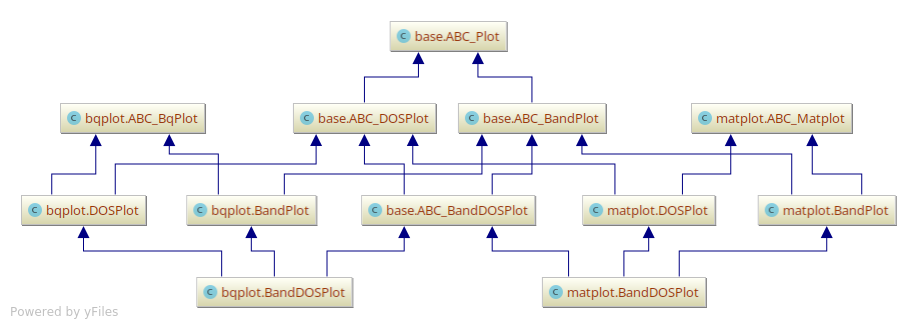
\includegraphics[width=1.1\linewidth]{img/pycharm_uml/matplot.png}}% Shorthand
\begin{frame}\frametitle{Visualization Module}
    \begin{itemize}
    \item<1-> Combine \emph{Python ABC} and \emph{multiple inheritance}
    \item<2-> \faArrowRight{} maximizes code reuse for different applications
        and viz. libraries employed
    \end{itemize}    
    \visible<3->{\centerline{\theimage}}
\end{frame}

\subsection{Desktop Frontend}
\label{sec:desktop-frontend}

\begin{frame}\frametitle{Desktop Frontend}
    Choice of GUI Toolkit: \textbf{TKinter} over (Kivy, PySide/PyQt, ...)

    Choice of Plotting tool: \textbf{matplotlib}
\end{frame}

\subsection{Web Frontend}
\label{sec:web-frontend}

\renewcommand{\theimage}{\includegraphics[width=1.0\linewidth]{img/py-viz-landscape.png}}% Shorthand
\begin{frame}\frametitle{Web Frontend}
    \visible<1->{The Python Visualization Landscape as of 2017...}
    \visible<2->{
      \centerline{\theimage}
      \begin{tiny}
          \href{https://github.com/rougier/python-visualization-landscape}{Python
            Visualization Landscape} by \href{https://github.com/rougier}{rougier} / BSD-2    
      \end{tiny}} 
\end{frame}

\begin{frame}\frametitle{Web Frontend}
    \begin{itemize}
    \item<1->Needed: a \textbf{survey} of OSS Frameworks for building a Web
        Dashboard using \textbf{only} \logoPython{}.
    \item<2-> Selection Process: \emph{Framework supports...}
        \begin{itemize}
        \item<3-> I. \emph{... interactive graphical control
              elements ('widgets') to control plots}
        \item<4-> II. \emph{... easy deployment}
        \item<5-> III. \emph{... some actual plotting libraries}
        \end{itemize}        
    \end{itemize}
\end{frame}

\begin{frame}\frametitle{Web Frontend}
    \begin{table}
        \resizebox{\textwidth}{!}{%
          \begin{tabular}{c||c|c|c|c}
            \visible<1->{I. \textbf{Widgets} & \logoJupyter{} jupyter & pyviz \logoPanel{} panel & \logoBokeh{} bokeh & \logoDash{} dash \\\hline
            Languages & \logoPython{} & \logoPython{} & \logoPython{} / \logoJavascript{} & \logoPython{} / \logoJavascript{} \\\hline}
            \visible<2->{II. \textbf{Deployment} & & & & \\
            - Jupyter & \faCheck{} & \faCheck{} & \faCheck{} & \faCheck{} \\
            - Standalone\footnote{Excluded: writing from scratch using Flask} & (\logoBinder{}, \logoDocker{})\footnote{workaround. See also: \href{https://github.com/oschuett/appmode}{appmode}, \href{https://github.com/QuantStack/voila}{voila}, \href{https://github.com/minrk/thebelab}{thebelab}} & \logoBokeh{} server & \logoBokeh{} server & \logoPlotly{} plotly \\\hline}
            \visible<3->{III. \textbf{Plots}\footnote{interactive only}  & & & & \\
            - 2D & \logoMatplotlib{} mpl, bqplot, \textbf{all}  \faArrowLeft{} & \logoHvplot{} hvplot,  \faArrowRight{} \textbf{most} \faArrowLeft{}  & \logoBokeh{} & \logoPlotly{}\\
            - 3D & ipyvolume, \textbf{all}  \faArrowLeft{} & \faClose{} & \logoBokeh{} & \logoPlotly{}}
          \end{tabular}
        }
    \end{table}
\end{frame}
% Talking Notes:
% - Our decision:
%   - PyViz best (abstract GUI declaration supports Tkinter) but no 3D for atom plots, so out again
%   - Jupyter > (Bokeh, Dash) but expect deployment in AiiDAlab (JupyterHub) so simpler
%   - problem: standalone will now be harder, but maybe possible through binder
%   - 2D: matplotlib first cause same as Tkinter, for now
%   
 







% 


\chapter{Applications}
\label{chap:applications}


To illustrate the use of the graphical user interface, two different physical
applications are shown in the desktop and the web frontend, respectively. From
the physics point of view, the example in the desktop version focuses more on the
density of states and the visualization of spin contributions, while the dataset
in web frontend focuses on the band structure $E(k)$ and the visualization
of defect states in supercells.

\section{Web Frontend: $\textrm{MoSe}_2$ Crystal}

Figure \textbf{TODO} shows the visualization of a band structure calculation of a 3 dimensional Molybdenum diselenide ($\textrm{MoSe}_2$ bulk) crystal using the default settings of the GUI. Even with the default settings the band structure plots clearly indicate, that $MoSe_2$ is a semiconductor, since there are no states at the Fermi level. Because the minimum of the conduction band is located at an other $k$ as the maximum of the valence band, the plot shows that $\textrm{MoSe}_2$ has an indirect band gap. This indicates that for the transition with the smallest energy difference between valence and the conduction band, both, energy and momentum have to change.

In contrast to the 3 dimensional extended $MoSe_2$ crystal, a $MoSe_2$ monolayer (see Fig. \textbf{TODO}) has a direct band gap but is still a semiconductor. Furthermore, the $\textrm{MoSe}_2$ monolayer has a defect atom in every 9th unit cell and the DFT computation is therefore done in a $3 \times 3$ supercell to restore periodicity. This is the reason for the much greater number of states in the band structure plot. 

Since the Brillouin zone of the supercell is smaller than the Brillouin zone of the same crystal without the defect, the supercell Brillouin zone is unfolded to the same size as the Brillouin zone of the unperturbed lattice. To account for the fact that the defect is only present in every 9th cell and its relative importance for the spectrum is therefore degraded, an unfolding weight is introduced to visualize the relative importance of bands in the unfolded Brillouin zone. By default, the unfolding weight is used by our visualization tool, but it can gradually be turned off in order to highlight the impact of defect states. This is shown in figure \textbf{TODO}. To even better visualize the defect state, it would also be possible to select the atom group belonging the defect atoms only. In this example, the analysis with reduced band unfolding shows, that there are many more direct band gaps origination from the defect state.




\section{Desktop Frontend: $\textrm{Co}$ Crystal}


% bänder isonlieren schwierig....fleur update--> label der E eigenvlas

%$m^{*}$ and $v_{G}(\vec{k})$
\section{Derived physical Quantities: Differentiation}
The kind of datasets handled in the scope of the project did not lend themselves
readily to applications of automatic differentiation techniques. Nevertheless,
it is possible to derive meaningful physical quantities from the band structure
using numerical differentiation techniques.

The effective mass $m^{*}$ represents the mass, that an electron appears to have due to the inter-atomic forces in the crystal. At every $\vec{k}_0$, where $E(\vec{k})$ has a local extremum, $E(\vec{k})$ can be expanded in a Taylor series with a vanishing first order term $E(k) = E_0 + \frac{\partial E(\vec{k})}{\partial \vec{k}} \cdot (\vec{k}-\vec{k}_0)^2$. Comparing this to the dispersion relation of a free electron $E(\vec{k})_{free} = \frac{\hbar^2 \vec{k}^2}{2 m_e}$ motivates the general definition 

\begin{equation}
    m^{*}_{k_i,k_j} = \hbar^2  \left(\frac{\partial^2E(\vec{k})}{\partial k_i \partial k_j}\right)^{-1}
\end{equation}

Since $\frac{\partial^2E(k)}{\partial \vec{k}_i \partial \vec{k}_j}$ depends on the direction of the partial derivatives, $m^{*}\big|_{i,j}$ is a tensor. Because the band structure files only contain a discrete sampled path in the Brillouin zone, only the derivatives that correspond to the direction from one high-symmetry point to the next can be computed. We are only interested in the diagonal terms of $m^{*}\big|_{i,j}$.

%maybe something about the directional dependency --> m is tensor...


A second potentially interesting quantity is the group velocity $v_{G}(\vec{k})$ associated to each band. The group velocity $v_{G}(\vec{k})$ at the Fermi energy $E = E_F$ is called Fermi velocity.

\begin{equation}
    v_{G}(\vec{k})\big|_i = \frac{1}{\hbar}\frac{\partial E(\vec{k})}{\partial \vec{k_i}}
\end{equation}


\subsection{Differentiation}

Since the k-mesh in DFT calculations is potentially very sparse, low order finite difference schemes are not expected to work well. Alternatively, one way to exploit all data points efficiently is to use fast Fourier transform methods, which are equivalent to the derivation of a truncated Fourier series. This method is expected be well-suited for the problem since the graph of the band structure $(k, E(|k|))$ with $k \in \{-\Gamma,..., H,..., \Gamma\}$ is periodic, where $\Gamma$ and $H$ are arbitrary representatives of the high symmetry points. This periodicity in the reciprocal space is a direct consequence of the periodicity of the crystal.

In Fourier space, spatial derivatives transform into multiplications, which can easily be shown by partial integration.

\begin{equation}
    f^{(n)}(x) = \mathcal{F}^{-1}\left((ik)^n\mathcal{F}(f(x))\right)
\end{equation}
 
To test the FFT differentiation method, a band was selected that did not have intersections with other bands within the interval between two high symmetry points and a stationary point at the high symmetry points. Then a resolution study was done to investigate the impact of the number of points within the interval.

The comparison between the FFT and a first-order central difference approximation of the second derivative (FD) is shown in Fig. \textbf{TODO}, where different k-mesh resolutions are compared to a derivative that is almost fully converged. The comparison indicates that for small N, the error of the FFT method is significantly smaller than the error of the FD derivative. This is especially striking in the vicinity of the high symmetry points, where the error of the differentiation is required to be small in order to get good approximations for $m^{*}$, which is only meaningful close to the high symmetry points.

When using more points, the difference between both approximation schemes is not significant. It is interesting to note, that the FFT method does not work anymore in the limit of extremely many points. In this case the derivative is dominated by Gibbs oscillations. These are most likely caused by small discontinuities in $E(k)$, due to basis changes inside the DFT computation.

At the current state the question remains to be answered weather the computation of $m^{*}$ and $v_g$ is useful. The number of bands, which the computation can be applied to is extremely limited. Since the bands in the data files are not labeled according to their corresponding eigenfunction but sorted by value, there are discontinuities at each point, where two bands intersect. This problem might be solved in the future. 













 %   \item Effective mass, that an electon in a crystal appears to have compared to a free %electron (due to interactions in the solid)
%    $m^{*} = \hbar^2  \left(\frac{\partial^2E(k)}{\partial k^2}\right)^{-1}$
%    \
%    \item Group velocity:
%    $v_{G}(\vec{k}) = \frac{1}{\hbar}\frac{\partial E(\vec{k})}{\partial \vec{k}}$%
%
%    
%    \item Problem: sparse k-Point mesh, but periodic band structure
%    \item Idea: Using FFT to compute accurate derivates:
%    \newline $\Leftrightarrow$ Differentiate a finite Fourier series
%    \newline $f^{(n)}(x) = \mathcal{F}^{-1}\left((ik)^n\mathcal{F}(f(x))\right)$


%%% Local Variables:
%%% mode: latex
%%% TeX-master: "../report"
%%% End:


\chapter{Conclusion}
\label{chap:conclusion}

\section{Outlook}
\label{sec:outlook}


\textbf{TODO} Module design:
- preprocessor module:
- desktop frontends:
  - PyViz Param \cite{pyviz-param} makes it possible to decouple the formal
  description of a particular GUI from the GUI library used. This would serve to
  separate interface and implementation like it is done in the preprocessor and
  visualization submodules. 


%%% Local Variables:
%%% mode: latex
%%% TeX-master: "../report"
%%% End:


\begin{appendices} 

\chapter{Manual}
\label{cha:manual}

The project code and documentation is hosted on the \texttt{masci-tools}
repository \cite{masci-tools} under the branch
\href{https://github.com/JuDFTteam/masci-tools/tree/studentproject18ws}{\texttt{studentproject18ws}}.
All of the project code resides in the folders \texttt{binder} (for the Web
Frontend Demo) and \texttt{studentproject18w} (all code and documentation). The
\texttt{README.md} serves as the manual. Therefore, the remaining part of this
chapter is a \TeX{}-ified version of that \texttt{README.md}.

\vspace{3em}
\hdashrule{\textwidth}{2pt}{2pt}
%% BEGIN TEXIFIED README ========================================
%%
%% Command to TeXify README.md from masci-tools/studentproject18ws:
%% pandoc -s README.md -o README.tex
%%
%% Manual changes needed after TeXification:
%% - remove badges on top (binder badge, ...)
%% - 'try it out here on': convert to ordinary link without binder badge image
%% - figure -> figure*
%% - texttt{long} -> path{long} (enables linebreak)
%% - replace code sections 'Tok' with lstlisting:
%%   \begin{lstlisting}[language=python, style=code]
%% \end{lstlisting}
%%

SiScLab 2018 Student Project \textbf{Analysis Tool for Materials
Design}. Written in Python3.

Authors: \href{https://github.com/Irratzo}{Johannes Wasmer},
\href{https://github.com/ChristianPartmann}{Christian Partmann}, and
\href{https://github.com/PraneethKatta}{Praneeth Katta}.

\section{Overview}\label{overview}

This subfolder \texttt{studentproject18ws} is currently a largely
independent side-project accompanying the main module
\texttt{masci-tools}. It was created in a student project, and consists
of three submodules:

\begin{itemize}
\tightlist
\item
  preprocessor: a HDF reader interface, and one implementation for
  \href{http://www.judft.de}{Fleur} band structure simulation output
\item
  visualization: a plotting interface, and one implementation for
  \href{http://www.judft.de}{Fleur} bandstructure+DOS plots
\item
  frontends: a Desktop GUI and a Web Dashboard (Tk and Jupyter) for
  interactive Fleur bandDOS plots.
\end{itemize}

A more thorough description and example use cases can be found in the
project \href{./doc/report.pdf}{report} and
\href{./doc/presentation.pdf}{presentation}.

\begin{figure*}
\centering
\includegraphics{./readme/web_frontend.png}
\caption{}
\end{figure*}

\section{For Frontend Users}\label{for-frontend-users}

\subsection{General Remarks}\label{general-remarks}

These remarks apply to all frontends.

Though the Desktop and Web Frontend are functionally identical, there
might be small differences in how the controls are used and how they are
labeled.

\subsubsection{File Input}\label{file-input}

The frontends currently expects band structure data in the HDF output
format of \href{http://www.judft.de}{Fleur}. The density of states data
is expected to be in the CSV output format of
\href{http://www.judft.de}{Fleur}, one file per spin. If no density of
states files are supplied, the frontend will just draw a band structure
plot (BandPlot) and omit the adjoined density of states plot (DOSPlot).
Thus, in the following BandDOSPlot stands for both kinds of plot. The
Web Frontend will only show controls for data that is present in the
input (e.g., DOS and spin controls).

\subsection{Desktop Frontend}\label{desktop-frontend}

\subsubsection{Installation}\label{installation}

A windows executable file (.exe) is made by packing all the required
packages into the file. Any modern PC running on windows can run the
frontend without any installation process and there is no prerequisite
to execute this executable file. PC need not have python or other
packages installed.

For executables for other operating systems, please contact the
developers.

\subsubsection{Usage}\label{usage}

Desktop based front end GUI is easy to use. By just running the .exe
file provided will open the software with the packages involved to run
the software. There are three tabs/windows in the software. In the first
tab, absolute paths to the input data files must be entered in this
order: HDF and (optional) DOS file for spin `0' and `1'.

Controls for all plots:

\begin{itemize}
\tightlist
\item
  Atom Groups: draw the BandDOSPlot only for the selected symmetry
  groups.
\item
  Character: select one or more band Characters (orbitals)
  `S',`P',`D',`F'.
\item
  Spin: select any one spin or both spins.
\item
  Marker size: Default marker size of 1.0 is selected. How ever, user
  have a choice to increase the marker size of the dots (eigenenergies)
  plotted in the BandPlot.
\item
  Ymin, Ymax: This control is used to limit the range energy range of
  the BandDOSPlot.
\item
  BandMin, BandMax: This control is used to limit the band range of the
  BandDOSPlot.
\item
  Update, SaveButton: Update the BandDOSPlot to the newly selected data
  by user. Save the the plot as a PDF on disk.
\item
  Exponential weight: The unfolding exponent for supercell calculations
  (see \href{./doc/report.pdf}{report}). Value 0.0 means no unfolding.
  If the calculation is done with a unit cell, this control has no
  effect.
\item
  Compare 2Characters: When a user wants to compare 2 characters, this
  button makes the BandPlot show the influence of each character to each
  eigenergy using a sequential (2) colormap. The control is disabled if
  other than two characters are selected.
\item
  Ignore Atom group: This button allows an option to ignore the atom
  groups.
\end{itemize}

Controls for the DOSPlot only:

\begin{itemize}
\tightlist
\item
  Select groups: include selected atom groups in the DOS
\item
  Interstitial: include the interstitial in the DOS
\item
  All characters: include all characters in the DOS regardless of
  character selection. In the DOS CSV file, different input data is used
  (a summed column).
\end{itemize}

After the Update button is clicked, a BandPlot or BandDOS plot is
produced in Tab 2. A 3D atomic plot is produced in Tab 3.

\subsubsection{Troubleshooting}\label{troubleshooting}

If the BandPlot is not visible:

\begin{itemize}
\tightlist
\item
  Check if the three input files (if any) are belonging to the same
  Fleur calculation and selected appropriately.
\item
  Check if at least one Atom Group, one Character, one Spin is selected.
\item
  Check if Ymin is less than Ymax and similarly BandMin is less than
  BandMax such that software is able to plot.
\end{itemize}

Click on Update once again. If problem persists, restarting of the
software would be last attempt for making it work. Please open an issue
or contact the developers if the problem persists.

\subsection{Web Frontend}\label{web-frontend}

\subsubsection{Access}\label{access}

The Web Frontend is a Jupyter Dashboard. It is in experimental state (no
fileupload yet). You can try it out
\href{https://mybinder.org/v2/gh/JuDFTteam/masci-tools/studentproject18ws?filepath=studentproject18w\%2Ffrontend\%2Fjupyter\%2Fdemo\%2Fbinder_demo.ipynb}{here
on Binder}. You can run it locally (see developer section). If you have
an {[}AiiDaLab
account{]}(https://aiidalab.materialscloud.org/hub/login**: the
dashboard is planned to be published as an app there.

\subsubsection{Usage}\label{usage-1}

Using the Dashboard should be self-explanatory to the domain user. Some
tips:

\begin{itemize}
\tightlist
\item
  unlike the Desktop frontend, plot updates are instantaneous.
\item
  multi-selection boxes: use ctrl or shift to select multiple items.
\item
  slider values can also be typed into the adjoining text box.
\item
  should the app ever appear to get stuck, a reload/rerun will do the
  trick.
\item
  unlike the Desktop Frontend, empty selections are impossible.
\end{itemize}

\section{For Developers}\label{for-developers}

\subsection{Installation}\label{installation-1}

Though \texttt{masci-tools} is availabe via PyPI, there is currently no
plan to integrate \texttt{studentproject18ws}. If you want to use it in
your code, clone the repo, use it in an IDE, or append the path to your
\texttt{sys.path}:

\begin{lstlisting}[language=bash, style=code]
import sys
if path_repo not in sys.path:
    sys.path.append(path_repo)
    
# now import works
from studentproject18w.hdf.reader import Reader
# ...
\end{lstlisting}

\subsubsection{Create project virtual
environment}\label{create-project-virtual-environment}

With conda (recommended): -
\href{https://www.anaconda.com/download}{Install Anaconda (3
recommended)} - Install the environment \texttt{masci-stupro} with the
necessary and recommended dependencies:

\begin{lstlisting}[language=bash, style=code]
conda create -f environment.yml
source activate masci-stupro
\end{lstlisting}

With virtualenv (untested):

\begin{lstlisting}[language=bash, style=code]
virtualenv masci-stupro
source masci-stupro/bin/activate
pip install -r requirements_pip.txt # install requirements
\end{lstlisting}

\subsection{Programmatic use}\label{programmatic-use}

In this example, a Fleur HDF file is preprocessed using the Recipe
\texttt{FleurBands}. The resulting output \texttt{data} with the
extracted and transformed HDF datasets and attached load methods
(Extract-Transform-Load) is then passed to a plotter, alongside some DOS
CSV files for a bandstructure plot using \texttt{matplotlib} as backend
library.

\begin{lstlisting}[language=python, style=code]
import matplotlib.pyplot as plt
from studentproject18w.hdf.reader import Reader
from studentproject18w.hdf.recipes import Recipes
from studentproject18w.plot.matplot import BandDOSPlot

data = None
reader = Reader(filepath=filepath_hdf)
with reader as h5file:
    data = reader.read(recipe=Recipes.FleurBands)
    #
    # Note:
    # Inside the with statement (context manager),
    # all data attributes that are type h5py Dataset are available (in-file access)
    # When the statement is left,the HDF5 file gets closed and the datasets are closed.
    #
    # Use data outside the with-statement (in-memory access: all HDF5 datasets converted to numpy ndarrays):
    data.move_datasets_to_memory()

plotter = BandDOSPlot(plt, data, filepaths_dos)
(fig, ax_bands, ax_dos) = plter.setup_figure(fig_ratio=[12,6], fig_scale=1, fig_title="BandDOS")
data_selection = some_selection_process()
plotter.plot_bandDOS(*data_selection)
plt.show()
\end{lstlisting}

\subsection{Try out Web Frontend
locally}\label{try-out-web-frontend-locally}

The demo notebook with the Dashboard is
\path{studentproject18w/frontend/jupyter/demo/demo.ipynb}.

\subsubsection{If using Jupyter
Notebook}\label{if-using-jupyter-notebook}

If using Windows, omit keyword \texttt{source}.

\begin{lstlisting}[language=bash, style=code]
source activate masci-stupro
cd mypath/masci-tools/studentproject18ws/
jupyter-notebook .
# if Home is not set to this dir, try this instead:
# /home/you/anaconda3/envs/myenv/bin/python /home/you/anaconda3/envs/myenv/bin/jupyter-notebook .
\end{lstlisting}

\subsubsection{If using Jupyter Lab}\label{if-using-jupyter-lab}

Additional installation step needed:

\begin{lstlisting}[language=bash, style=code]
source activate masci-stupro
jupyter labextension install @jupyter-widgets/jupyterlab-manager jupyter-matplotlib ipyvolume
cd mypath/masci-tools/studentproject18ws/
jupyter-lab
\end{lstlisting}

\subsection{Frontend Deployment}\label{frontend-deployment}

\subsubsection{Desktop Frontend}\label{desktop-frontend-1}

To create executables for different operating systems, use
\href{https://www.pyinstaller.org/}{PyInstaller}. The target file is
\texttt{frontend/tkinter/gui.py}.

\subsubsection{Web Frontend}\label{web-frontend-1}

The Web Frontend is currently a single Jupyter Notebook. In order to
publish it as a usable standalone app, additional work has to be done.

\begin{itemize}
\tightlist
\item
  (recommended: create \texttt{frontend/jupyter/Dashboard.py} widget and
  put code of
  \href{./frontend/jupyter/demo/demo_backend.ipynb}{demo\_back.ipynb}
  notebook inside it. Use
  \href{https://github.com/aiidalab/aiidalab-widgets-base/blob/master/aiidalab_widgets_base/structures.py}{aiidalab-widgets-base
  \textgreater{} StructureUploadWidget} as a template. Create
  \texttt{frontend/jupyter/Dashboard.ipynb} notebook. Use
  \href{https://github.com/aiidalab/aiidalab-widgets-base/blob/master/structures.ipynb}{StructureUploadWidget
  Demo Notebook} as a template.)
\item
  Add \href{https://pypi.org/project/fileupload/}{fileupload} to widget
  (again, like in StructureUploadWidget. See
  \href{./frontend/jupyter/demo/binder_fileupload_test.ipynb}{binder\_fileupload\_test.ipynb}
  notebook for a demo that works with binder.)
\item
  Now the Web Frontend should work on Binder.
\item
  For publishing the app on AiiDA Lab, the app has to be registered in
  the
  \href{https://github.com/aiidalab/aiidalab-registry}{aiidalab-registry}.

  \begin{itemize}
  \tightlist
  \item
    The project code is in Python3, but aiidalab requires Python2. So
    the code has to first be backported by hand using the `future**
    package. If this takes too long, maybe try the tool
    \href{https://pypi.org/project/3to2/}{3to2}.
  \item
    Use the simplest app in the registry,
    \href{https://github.com/aiidalab/aiidalab-units}{aiidalab-units} as
    a template. Adapt code.
  \item
    Try it out first in the
    \href{https://www.materialscloud.org/work/quantum-mobile}{Quantum
    Mobile Virtual Machine}, which has aiidalab installed and
    configured. Else try it in a virtual environment with
    \href{https://pypi.org/project/aiidalab/}{aiidalab} installed from
    PyPI.
  \item
    Register the app.
  \end{itemize}
\end{itemize}

Note: other publishing options besides Binder and AiiDALab are listed
\href{https://github.com/markusschanta/awesome-jupyter}{here}. For
instance, \href{http://colab.research.google.com/}{Google Colaboratory}
is a free Notebook hosting service that allows file upload.

\subsection{Exending the code}\label{exending-the-code}

\subsubsection{Use Case: HDF with DOS data
included}\label{use-case-hdf-with-dos-data-included}

The Fleur output HDF format is expected to change and incorporate more
data. In turn, this project's code has to be extended as well. The
procedure is outlined for a an example use case: the incorporation of
DOS data into the band structure HDF (thus eliminating the need for
separate DOS CSV files). The instructions show how to extend the
preprocessor, the visualization and frontend submodules to that
scenarion.

\begin{itemize}
\tightlist
\item
  Add a new output type to \texttt{hdf/output\_types}, say
  \texttt{FleurBandDOS}. Let it inherit from output type
  \texttt{FleurBands}. If you want an output type just for the DOS as
  well, add a type \texttt{FleurDOS} and let \texttt{FleurBandDOS}
  inherit it.
\item
  Add a new recipe to \texttt{hdf/recipes} e.g. \texttt{FleurBandDOS}.
  Copy unchanged things from recipe \texttt{FleurBands}.
\item
  If needed, add new transforms to \texttt{hdf/input\_transforms}.
  Adhere to the transform function standard there. If there are mutual
  dependencies, add them to the list in the top of the file.
\item
  Add a DOS data selection method to the output type
  \texttt{FleurBands}. The \texttt{DOSPlot} in \texttt{plot/base} types
  will need those to plot the DOS plot. Simply adapt from the function
  in \texttt{dos/reader} for the DOS CSV files, adopt the identical
  signature.
\item
  In the \texttt{DOSPlot} types in submodule \texttt{plot}, add a switch
  to the constructor that can distinguish the three cases (bands,
  bands+CSV DOS, bands+HDF DOS). Use the switch in the \texttt{plotDOS}
  methods, and for the case bands+HDF DOS, call your new
  \texttt{FleurBandDOS} function.
\end{itemize}

\subsubsection{Extending the Visualization
(Plots)}\label{extending-the-visualization-plots}

\begin{itemize}
\tightlist
\item
  In addition to the inheritance scheme based on Python
  \texttt{AbstractBaseClass} (ABC) detailed in the
  \href{./doc/report.pdf}{report}, the \texttt{Plot} types in
  \texttt{plot} have an additional facility that helps to keep the
  appearance of different Frontends synchronized: each type has an
  attribute \texttt{icdv} of type
  \texttt{InteractiveControlDisplayValues}. This is an ABC with the same
  inheritance as the application Plot types. For every plot control
  argument that an application type's Plot type exposes in it's methods'
  signatures, this attribute describes the parameters of the
  accompanying control widget in the Frontend text label, default
  values, value ranges, and so on. In the current code, only the Web
  Frontend uses this facility, so the labels in the Desktop Frontend
  differ slightly.\\
\item
  It is worth pointing out that unlike other languages, Python does not
  enforce implemented abstract methods to have the same method
  signature. However, when a new implementation for a different plotting
  library/backend is added, it is recommended to adopt the
  \texttt{abstractmethod} signature. That way, changing the backend in a
  use case only requires to change the import.
\end{itemize}




%% FINISH TEXIFIED MANUAL ========================================
\hdashrule{\textwidth}{2pt}{2pt}






%% =========================================================
%%% Manuals Chapter OLD VERSION ============================
%% =========================================================
% \section{Frontends User Manual}
% \label{sec:user-manual}

% \subsection{System Requirements \& Installation}
% \label{sec:system-requirements}

% The Desktop Frontend is distributed as an executable file. 

% \subsection{Input Data Formats}
% \label{sec:input-data-formats}

% \subsection{GUI Usage}
% \label{sec:gui-usage}

% The Desktop and Web Frontend are functionally identical and use the same
% graphical descriptors. Thus these points hold true for both alike.

% Instead of dragging the sliders, values can be typed into their adjoining value
% displays as well.

% \textbf{TODO}: web frontend: binder or colab link

% \subsection{Troubleshooting}
% \label{sec:troubleshooting}


% \section{Developer Manual}
% \label{sec:developer-manual}

% At the time of this report, the package is written in Python 3. It is hosted on
% the \texttt{masci-tools} repository \cite{masci-tools} under the branch
% \href{https://github.com/JuDFTteam/masci-tools/tree/studentproject18ws}{\texttt{studentproject18ws}}.
% All of the project code resides in the folders \texttt{binder} (for the Web
% Frontend; see below) and \texttt{studentproject18w} (all code and
% documentation). The \texttt{README.md} contains the same installation
% instructions listed here.

% \subsection{Creating the project virtual environment}
% \label{sec:creat-proj-virt}

% \begin{lstlisting}[language=bash, style=code]
%     # if using conda (recommended)
%     conda create -f environment.yml
%     source activate 

%     # if using pip (untested)
    
% \end{lstlisting}

% \subsection{Creating Desktop Frontend Executables}
% \label{sec:creat-deskt-front}



% \subsection{Extending the Preprocessor}
% \label{sec:extend-prepr}

% \subsection{Extending the Visualization \& Frontends}
% \label{sec:extend-visu-}

% \textbf{TODO:} publish on aiidalab 

% \textbf{TODO:} hosting alternatives
% \begin{itemize}
% \item binder with example
% \item google colab (see jupy wiki or jupy awesome) \cite{jupyter-awesome}
% \item voila?
% \end{itemize}







%%% Local Variables:
%%% mode: latex
%%% TeX-master: "../report"
%%% End:

\end{appendices}   


% % Original template (biblatex):
% \appendix

% % Original template (biblatex):
% \bibliographystyle{authoryear-fr}
% \bibliographystyle{authoryear}
% \bibliography{references}

% Adapted template (biber):
\printbibliography

% \clearpage

%%%%%%%%%%%%%%%% 
%%% Abstract %%%
%%%%%%%%%%%%%%%% 

\thispagestyle{empty}

\vspace*{\fill}
\noindent\rule[2pt]{\textwidth}{0.5pt}\\
{\textbf{Abstract ---}}
In this project, the raw data of the DFT simulations from Fleur are read, pre-processed and stored in suitable variables, then  extracted various features from the data from the DFT simulations such as Fermi velocity, Effective mass. Then this data is visualized using suitable color pots for a physicist to understand the plots, material characteristics using the plots. This API is converted into a frontend GUI for easier use in future. The overall project helps physicists to solve their problem of reading the DFT simulations data.

{\textbf{Keywords}}
Fleur, DFT Simulations, visualization, Front end GUI, Feature extraction.
\\
\noindent\rule[2pt]{\textwidth}{0.5pt}
\begin{center}
    AICES\\
    Schinkelstr. 2\\
    Rogowski Building\\
    4th Floor\\
    52062 Aachen    
\end{center}
\vspace*{\fill}

%%% Local Variables:
%%% mode: latex
%%% TeX-master: "report"
%%% End:
                % original template

\end{document}
%%% Local Variables:
%%% mode: latex
%%% TeX-master: t
%%% End:
